\section{Implementation}
\label{sec:implementation}

The objective of the compression algorithm is to reduce amount of data representing FEM results and also the ability to reconstruct original data from its smaller representation. This saves storage capacity and also accelerates data transfer between computers as the analysis itself and the post-processing of results is usually done on different work stations.

Compression method can be lossy or lossless based on quality of data reconstructed of its compressed representation. Lossless methods are able to fully reconstruct original data. Lossy methods on the other hand produce only approximations of original data. 

SVD is used as part of the compression algorithm. SVD method applied to arbitrary matrix produces decomposition that consist of corresponding singular values and singular vectors. This process is fully reversible (with the assumption that the numerical errors are negligible). The original matrix can be reconstructed by the multiplication of decomposed parts. However, the compression algorithm is based on modification of decomposition to create low-rank approximation matrix. The reconstructed matrix slightly differs from the original matrix and algorithm therefore does lossy compression.

SVD decomposition is applied on matrices. The first thing to do is therefore to assemble an input matrix. Results from the Finite element method are discrete values calculated in nodes or integration points. There are usually multiple fields in result data (e.g. displacements, stress, strain etc.) and each field can have multiple components (e.g. displacements can have $X$, $Y$ and $Z$ component). As non-linear analyses usually lead to multiple computation steps there are multiple sets of data per each field component. All data corresponding to a single field component form the input matrix $\mtrx{A}$ to the compression algorithm. Only single field component is considered to fill the input matrix $\mtrx{A}$. Results for different data components (even for the same field) can be independent from each other. There can also be order-of-magnitude difference between the components and the compression algorithm could potentially clear the important information in the weaker component. Another reason against merging of components is computational complexity. The smaller the matrix $\mtrx{A}$ is, the faster the decomposition algorithm performs.

Each row of matrix $\mtrx{A}$ corresponds to single time step and each column corresponds to a single node or integration point. Once the matrix $\mtrx{A}$ is built for a field component the compression algorithm can be applied on it. It is purely algebraic procedure, no information about geometry of the mesh is needed. 

% The compression algorithm is based on low-rank approximation matrix created from SVD decomposition. Results for time steps are not independent. They usually have some relation between them. List of singular values produced by the SVD method reveals the dependency between the singular vectors that form the orthogonal base of the matrix $\mtrx{A}$.

\subsection{Low-rank approximation matrix}

From the definition of SVD in (\ref{eq:svd-def}) and from the properties of SVD presented in section \ref{sec:math} follows the fact that a matrix can be represented in the form of its SVD components as a sum of rank-1 matrices in the form

\begin{equation}
\mtrx{A}=\mtrx{U_{1}}S_{1}\mtrx{V_{1}^{T}}+\mtrx{U_{2}}S_{2}\mtrx{V_{2}^{T}}+ ... +\mtrx{U_{n}}S_{n}\mtrx{V_{n}^{T}},
\label{eq:svd-expansion}
\end{equation}

\noindent
where $S_{i}$ is $i$-th singular value, $\mtrx{U_{i}}$ and $\mtrx{V_{i}}$ are corresponding singular vectors, and $n$ is the rank of matrix~$\mtrx{A}$. Considering the fact that singular values are ordered $S_{1} \geq S_{2} \geq S_{3} \geq ... \geq S_{n}$ the above formula implies that the first term would have the highest contribution and last term would have the lowest contribution to matrix~$\mtrx{A}$. Therefore, if we take only first $r$ members of the above summation we get an approximation matrix

\begin{equation}
\mtrx{A'}=\mtrx{U_{1}}S_{1}\mtrx{V_{1}^{T}}+\mtrx{U_{2}}S_{2}\mtrx{V_{2}^{T}}+ ... +\mtrx{U_{r}}S_{r}\mtrx{V_{r}^{T}}.
\label{eq:svd-approx-expansion}
\end{equation}

The quality of approximation depends on the magnitude of the singular values omitted from the approximation formula, namely $S_{r+1} ...  S_{n}$. The compression algorithm is based on assumption that the first singular value is order-of-magnitude higher than singular values at the end of the decomposition sequence. In special cases, when $r=n$, or $S_{i}=0$ for all $i \geq r$ the omitted singular values do not contribute to the sum and the compression is therefore lossless. In other cases, approximation error has to be calculated and taken into account to avoid loss of important details in data.

The main goal of the compression algorithm is to find a compromise between low approximation error and high compression ratio $CR$ which is calculated using the formula

\begin{equation}
CR=\frac{r(m+n+1)}{m n},
\label{eq:cr-def}
\end{equation}

\noindent
where $m$ and $n$ are dimensions of matrix $\mtrx{A}$. Explanation of the compression ratio formula is best done using Figure~\ref{fig:lowrank_svd}. Light color represents the part of matrix decomposition that is to be stored in the output file as a low-rank approximation of the input.

\begin{figure}[H]
\centering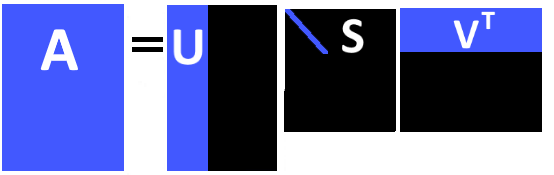
\includegraphics[width=0.7\textwidth]{figures/low_rank_decomposition_diagram}
\caption{Decomposition of input matrix $\mtrx{A}$ into diagonal matrix of singular values $\mtrx{\Sigma}$ and matrices of left and right singular vectors. Light color illustrates low-rank approximation.}
\label{fig:lowrank_svd}
\end{figure}

Let us assume that the matrix is not empty and has full-rank. Then from the formula above follows that if $r$ equals to the rank of matrix $\mtrx{A}$ the compression ratio is always higher than one. In other words the memory consumption of stored decomposition is bigger than the size of the original matrix. To make the compression algorithm applicable the parameter $r$ must conform to the condition

$$r<\frac{m n}{m+n+1}.$$

\noindent
Considering the usual shape of matrix containing FEM results this inequality is easily satisfiable even for the $r$ being close to the rank of the original matrix as in the typical case the number of nodes or integration-points is much higher than the number of analysis steps and therefore $m<<n$.

\subsection{Algorithm description}
Once the SVD decomposition is calculated the compression algorithm removes a certain number of singular values and corresponding singular vectors. The remaining singular values and vectors represent the compressed data. There are two strategies that influence the way how to get the number of singular values to be preserved -- resulting size and quality. Each strategy is assigned a control parameter that determines compression ratio or approximation error.

\paragraph{Compression ratio}
If the focus is only on the size of compressed data, the rank $r$ of the approximation matrix can be calculated by the formula

\begin{equation}
r=\ceil*{CR \times \frac{m n}{m+n+1}},
\end{equation}

\noindent
where $CR$ is the compression ratio, $0 \leq CR \leq 1$ ($0$ results in absolute compression while $1$ results in no compression).

\paragraph{Approximation error}
In the usual case the most important parameter to take into account is the approximation error. Algorithm is trying to minimize the compression ratio while at the same time ensuring that predefined limit of approximation error is not exceeded. To quantify the error the Mean squared error ($MSE$) metric is used. To be able to compare different data-sets having different scales the normalized version of $MSE$ is used - Normalized root-mean-square deviation ($NRMSD$). Both metrics are defined in section \ref{sec:error}.

But how can be the rank of approximation matrix effectively calculated from the desired approximation error? Here comes useful the interesting property of the singular values:

% TODO: Reference to source or further explanation needed. (prof. Marek?)

\begin{equation}
\sum_{i=1}^{m} \sum_{j=1}^{n} (\mtrx{A_{ij}})^{2} = \sum_{i=1}^{k}{\sigma_{i}^{2}},
\label{eq:elem-sqr-sigma-sqr}
\end{equation}

\noindent
where $k=min(m, n)$, i.e. the smallest of two dimensions of the matrix $\mtrx{M}$. The above formula states that the sum of squared elements of matrix $\mtrx{A}$ equals to the sum of squared singular values $\sigma_{i}$ of the same matrix $\mtrx{A}$.

Using formulas \eqref{eq:svd-expansion} and \eqref{eq:svd-approx-expansion} the equation \eqref{eq:elem-sqr-sigma-sqr} can be applied to the difference between original matrix $\mtrx{A}$ and approximation matrix $\mtrx{A'}$.

\begin{equation}
\sum_{i=1}^{m} \sum_{j=1}^{n} (\mtrx{A_{ij}} - \mtrx{A'_{ij}})^{2} = \sum_{i=r+1}^{k}{\sigma_{i}^{2}},
\end{equation}

\noindent
where the term on the right-hand side is the sum of squares of those singular values of the matrix $A$ that are going to be cut away by the compression algorithm. The equation can be rewritten using the definition of $MSE$ in \eqref{eq:mse-def} to

\begin{equation}
MSE \times m n = \sigma_{r+1}^{2} + \sigma_{r+2}^{2} + ... + \sigma_{k-1}^{2} + \sigma_{k}^2
\end{equation}

\noindent
and using \eqref{eq:nrmsd-def} further to

\begin{equation}
(NRMSD \times (X_{max}-X_{min}))^{2} \times m n = \sigma_{r+1}^{2} + \sigma_{r+2}^{2} + ... + \sigma_{k-1}^{2} + \sigma_{k}^2.
\end{equation}

Then $NRMSD$ can be used as a quality metric for the compression algorithm because normalization makes it usable for different datasets. Calculation of rank of the approximation matrix is depicted as pseudo-code in algorithm \ref{alg:rank-calculation}. Algorithm uses the following inequality to test whether the desired rank has been reached

\begin{equation}
e > \frac{\sqrt[]{\frac{\sigma_{r+1}^{2} + \sigma_{r+2}^{2} + ... + \sigma_{k-1}^{2} + \sigma_{k}^2}{m n}}}{X_{max}-X_{min}},
\end{equation}

\noindent
where $e$ is NRMSD used as an error limit that can not be exceeded to achieve reasonable quality of approximation.

\begin{algorithm}
  \caption{Calculation of rank for approximation matrix from maximum allowed error}\label{rankAlgorithm}
  \label{alg:rank-calculation}
  \begin{algorithmic}[1]
  	\INPUT maximum allowed error ($e$), array with singular values ($S$), element count ($c$), maximum element value ($x_{max}$), minimum element value ($x_{min}$)
    \OUTPUT rank of resulting matrix
    \Procedure{CalculateRank}{$e, S, c, x_{max}, x_{min}$}
      \State $MSE \gets 0$
      \State $NRMSD \gets 0$
      \State $rank \gets S.length$
      \While{$NRMSD < e$}\Comment{repeat until max error is reached}
        \State $MSE \gets MSE + S[rank]/c$ \Comment{calculate MSE for current rank}
        \State $NRMSD \gets \sqrt{MSE} / (x_{max} - x_{min})$ \Comment{normalize error}
        \State $rank \gets rank - 1$ \Comment{decrement rank for next loop}
      \EndWhile
      \State \textbf{return} $rank + 1$ \Comment{Add one to not exceed maximum allowed error}
    \EndProcedure
  \end{algorithmic}
\end{algorithm}

\subsection{Optimization}

% http://mathoverflow.net/questions/161252/what-is-the-time-complexity-of-truncated-svd

Time complexity of the exact SVD decomposition algorithm is $O(m^2n)$, where $m<n$. This theoretical algorithm complexity is confirmed by two benchmarks where the dependency of execution time on varying matrix dimension is shown. The results of the benchmarks are depicted in Figure \ref{fig:ExeTime_rows} and Figure \ref{fig:ExeTime_columns}. Several observations were made from the results:

\begin{itemize}
\item The algorithm is most efficient in cases where one dimension of the input matrix is very low compared to the other. However, this is almost always the case when compressing results from FEM -- number of time steps seldom exceeds hundreds.
\item Moreover, time steps can be split into smaller ranges and the algorithm can be applied on each range separately. This will improve performance and can also increase quality of compression if the key time steps on the range boundaries are carefully selected.
\item Randomized SVD algorithm has the same order of algorithmic complexity but yet can help to significantly reduce execution time.
\end{itemize}

Storage size of SVD decomposition itself can also be optimized. $\mtrx{\Sigma}$ being a diagonal matrix can be stored as single list of singular values $\sigma_{i}$ or can be even multiplied with the matrix of left singular vectors $\mtrx{U}$.

% main features for optimization: key time steps (time step span compression), Randomized SVD, Parallelization, Sparse matrix of details, prenasobeni U matice singularnimi cisly, trochu usetrim pamet, mohu pouzit vzorkovani...
